% MA211 - Lecture 11
\documentclass[pdftex, xcolor=pdftex, dvipsnames,handout]{beamer}

\usetheme{MA211}
\usepackage{thumbpdf}
\usepackage{wasysym}
%\usepackage{ucs}
\usepackage[utf8]{inputenc}
\usepackage{pgf,pgfarrows,pgfnodes,pgfautomata,pgfheaps,pgfshade}
\usepackage{verbatim}

\usepackage{eurosym}
\usepackage{euler}

\usepackage{calc}               % Simple computations with LaTeX variables
%\usepackage[hang]{caption2}     % Improved captions

\usepackage{graphicx}           % Standard graphics package

\usepackage{amsmath, amsthm, amssymb}


\newcommand{\fquad}{\mbox{\qquad}}
\newcommand{\bull}{$\bullet$ }

\newcommand {\I} {\mathcal I}
\newcommand {\calI} {\mathcal I}
\def\disint{\displaystyle\int}

\DeclareMathOperator{\D}{d}
\newcommand{\dydx}{\frac{\D y}{\D x}}

%\definecolor{gray}{rgb}{0.69, 0.69, 0.69} \newcommand{\gray}[1]{\textcolor{gray}{#1}}
\definecolor{dogreen}{rgb}{0.33, 0.42, 0.18} \newcommand{\dogreen}[1]{\textcolor{dogreen}{#1}}
\definecolor{maroon}{rgb}{.5,0.2,0.2}\newcommand{\maroon}[1]{\textcolor{maroon}{#1}}
\definecolor{greena}{rgb}{.1,0.581,0.1}\newcommand{\greena}[1]{\textcolor{greena}{#1}}

\definecolor{blue4}{rgb}{0,0,.545}
\newcommand{\Blue}[1]{\textcolor{blue}{#1}}
\newcommand{\Red}[1]{\textcolor{red}{#1}}
\definecolor{pink}{rgb}{1.,0.75,0.8}
\definecolor{darkred}{rgb}{0.5,0.0,0.0}
\definecolor{darkgreen}{rgb}{0,0.3,0.3}
\definecolor{purple}{rgb}{0,0.3,0.3}
\definecolor{darkblue}{rgb}{0.0, 0.0, .5}
\definecolor{dpurple}{rgb}{.3,.0,.3}
\newcommand{\Green}[1]{\textcolor{darkgreen}{#1}}
\newcommand{\DRed}[1]{\textcolor{darkred}{#1}}
\newcommand{\DBlue}[1]{\textcolor{darkblue}{#1}}
\newcommand{\Purple}[1]{\textcolor{dpurple}{#1}}
\newcommand{\Emph}[1]{\textcolor{darkred}{\textbf{\it #1}}}
\newcommand{\remph}[1]{\textcolor{darkred}{\textbf{\emph{#1}}}}
\newcommand{\bemph}[1]{\textcolor{darkblue}{\textbf{\emph{#1}}}}
\newcommand{\gemph}[1]{\textcolor{darkgreen}{\textbf{\emph{#1}}}}
\newcommand{\Bf}[1]{\textcolor{darkblue}{\textbf{#1}}}
\newcommand{\Gf}[1]{\textcolor{darkgreen}{\textbf{#1}}}
\newcommand{\Rf}[1]{\textcolor{red}{\textbf{#1}}}
\newcommand{\Rmf}[1]{\textcolor{red}{\mathbf{#1}}}

\newcommand{\Conj}[1]{\overline{#1}}

\newcommand{\code}[1]{\textcolor{darkblue}{\texttt{\textbf{#1}}}}
\newcommand{\icode}[1]{{\blue\texttt{\textbf{\emph{#1}}}}}
\newcommand{\gcode}[1]{{\Green{\texttt{\textbf{\emph{#1}}}}}}
\newcommand{\out}[1]{\texttt{\emph{\textbf{\Green{#1}}}}}





\newenvironment{vminipage}%
{\begin{Sbox}\begin{minipage}\begin{small}\begin{verbatim}}%
{\end{verbatim}\end{small}\end{minipage}\end{Sbox}\fbox{\TheSbox}}

\newenvironment{nminipage}%
{\begin{Sbox}\begin{minipage}}%
{\end{minipage}\end{Sbox}\fbox{\TheSbox}}


\let\Arg\relax\DeclareMathOperator{\Arg}{\mathtt{Arg}}
\let\Arg\relax\DeclareMathOperator{\e}{\mathtt{e}}

\newcommand {\AND} {\wedge}
\newcommand {\OR} {\vee}
\newcommand {\NOT} {\neg}
\newcommand {\IMPLIES} {\rightarrow}
%\newcommand {\IFF} {\leftrightarrow}
\renewcommand {\iff} {\Leftrightarrow}
\newcommand {\NAND} {\uparrow}
\newcommand {\NOR} {\downarrow}
\newcommand {\XOR} {\otimes}

\newenvironment{citemize}% Colour items
{\begin{description}}%
{\end{description}}

\newcommand {\maroonitem}{\item[\maroon{$\bullet$}]}

\newcommand {\gitem} {\item {\includegraphics[width=.4cm,angle=-10]{img/green-bullet-on-white.ps}}}
\newcommand {\ritem} {\item {\includegraphics[width=.4cm,angle=-10]{img/red-bullet-on-white.ps}}}
\newcommand {\yitem} {\item {\includegraphics[width=.4cm,angle=-10]{img/yellow-bullet-on-white.ps}}}
\newcommand {\bitem} {\item {\includegraphics[width=.4cm,angle=-10]{img/blue-bullet-on-white.ps}}}

\newcommand {\greenitem} {\item {\includegraphics[width=.4cm,angle=-10]{img/green-bullet-on-white.ps}}}
\newcommand {\reditem} {\item {\includegraphics[width=.4cm,angle=-10]{img/red-bullet-on-white.ps}}}
\newcommand {\yellowitem} {\item {\includegraphics[width=.4cm,angle=-10]{img/yellow-bullet-on-white.ps}}}
\newcommand {\blueitem} {\item {\includegraphics[width=.4cm,angle=-10]{img/blue-bullet-on-white.ps}}}

\newcommand {\eq}[1]%
  {$\DBlue{#1}$}
\newcommand {\eqd}[1]%
  {$\displaystyle\DBlue{#1}$}
%\newcommand{\eq}[1]{\boldmath \DBlue{$#1$}}


\newcommand {\csf}{\centerslidesfalse}
\newcommand {\cst}{\centerslidestrue}

\newcommand {\vecii}[2] {   \big(\begin{smallmatrix} #1 \\ #2 \end{smallmatrix}\big)}
\newcommand{\atwo}[2]{\left(\!\!\begin{array}{c} #1 \\ #2 \end{array}\!\!\right)}


\newcommand{\C}{\mathbb{C}}
\newcommand{\Q}{\mathbb{Q}}
\newcommand{\R}{\mathbb{R}}
\newcommand{\N}{\mathbb{N}}
\newcommand{\Z}{\protect\mathbb{Z}}  % protect for index.
\newcommand {\Rs}{ \mathbb{R}}
\newcommand {\Cs}{ \mathbb{C}}
\newcommand {\Rnn}{ \mathbb{R}^{n \times n}}
\newcommand {\Rn}{ \mathbb{R}^{n}}


\newcommand{\mblock}{%
\setbeamercolor*{block title}{bg=maroon,fg=white}
\setbeamercolor*{block body}{bg=white,fg=maroon}
}%

\newcommand{\bblock}{%
\setbeamercolor*{block title}{bg=Steel,fg=white}
\setbeamercolor*{block body}{bg=Mylightgray,fg=Steel}
}%

\newcommand{\gblock}{%
\setbeamercolor*{block title}{bg=Green,fg=white}
\setbeamercolor*{block body}{bg=Mylightgray,fg=darkgreen}
}%


\newcommand{\rblock}{%
\setbeamercolor*{block title}{bg=Red,fg=white}
\setbeamercolor*{block body}{bg=white,fg=Black}
}%


\newcommand{\TakeNotes}{
\includegraphics[width=2cm]{TakeNote}}

\def\eps{\varepsilon}
\newcommand {\del}[2]{ {\frac{\partial #1}{\partial #2}}}
\newcommand {\x}[1]{x^{[#1]}}
\newcommand {\delx}{ {\frac{\partial}{\partial x}}}
\newcommand {\delt}{ {\frac{\partial}{\partial t}}}
\newcommand {\dely}{ {\frac{\partial}{\partial y}}}
\newcommand {\ith}{{(i)}}
\renewcommand {\vec}[1]{ {\boldsymbol{#1}}}
\newcommand {\Oh} {\mathcal O}
\newcommand {\Err} {\mathcal E}
%\newcommand {\th} {\mathrm{th}}
\DeclareMathOperator{\fl}{fl}
\DeclareMathOperator{\sign}{sign}
\DeclareMathOperator{\Cond}{Cond} 
\DeclareMathOperator{\cond}{cond}
\DeclareMathOperator{\diag}{diag} 
\DeclareMathOperator{\sym}{sym} 
\DeclareMathOperator{\Trace}{Trace}
%\DeclareMathOperator{\D}{d}
\DeclareMathOperator{\E}{e}

\newcommand {\Rsym}{{ \mathbb{R}^{n \times n}_\mathrm{sym}}}

\newcommand {\st} {\mathrm{st}}
\newcommand {\nd} {\mathrm{nd}}


\parskip .25cm


\theoremstyle{definition}
\newtheorem{exercise}{Exercise}[section]
\newtheorem{method}{Method}[section]

\newcommand{\Header}[1]{\begin{center}{\Large \Bf{#1}}\end{center}}

\subtitle{MA211}
\title{Lecture 11: The case \eq{D<0}}

\author{Dr Niall Madden}

\date{\Large Monday, $8^\mathrm{th}$ October  2008}


\begin{document}


\frame{

\begin{block}{}
\begin{center}
{\large \insertsubtitle}

\vspace{.1cm}

\begin{large}
\textbf{\inserttitle}
\end{large}

\vspace{.15cm}

% {\footnotesize \insertauthor}

\vspace{.3cm}

{ {\insertdate}}
\end{center}
\end{block}


\vspace{-0.25cm}
\begin{center}
%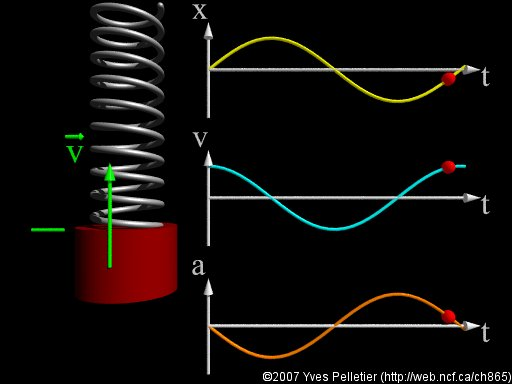
\includegraphics[height=4cm]{images/SHM.jpg}

\end{center}
}


\frame{

\Header{Class test on \alert{Wednesday}}

\Bf{Reminder:} There will be a 30 minute in-class test on Wednesday.

It will be worth approximately 5\% for total for MA211.


Questions will be based on \Bf{Problem Set 2}.






}

\frame{
  \frametitle{In this class...}

%\begin{columns}[c]
%\column{0.5\textwidth}
%\begin{small}
 \tableofcontents
%\end{small}

%\column{0.5\textwidth}
For more details, see \Bf{17.1 } of Stewart.

%\end{columns}

}



\section{Recall...}



\frame{

\begin{center}
{\large \Emph{2nd Order, Constant Coefficient, Homogeneous
    DEs}}
\end{center}

Last week we started on solving problems of the form
\begin{block}{}
\[ a y''(x) + by'(x) + cy(x) =0.\]
where \eq{a}, \eq{b} and \eq{c} are constants (real numbers).
\end{block}

We introduced the \Emph{The Auxiliary Equation}:
\[ aR^2 + bR + c=0,\]
and the \Bf{Discriminant}, \eq{D=b^2 -4ac}.

We use a different approaches depending on if 
\begin{center}
(i) \eq{D>0},  \qquad \qquad  (ii)  \eq{D=0}  \qquad\qquad (iii) \eq{D<0}.
\end{center}


}

\subsection{$D>0$}
\rblock
\frame{

The easiest case is \eq{D=b^2 -4ac>0}.
\begin{block}{$D>0$}
If \eq{D=b^2 -4ac>0}, then the auxiliary equation
\[ ar^2 + br + c=0\]
has two solutions:
\[
R_1 = \frac{-b + \sqrt{b^2 -4ac}}{2a}, \qquad
R_2 = \frac{-b - \sqrt{b^2 -4ac}}{2a}, 
\]
and the general solution is
\[
y (x) = A e^{R_1x} + B e^{R_2x}.
\]
\end{block}

}


\rblock
\subsection{$D=0$}
\frame{
The next easiest case is \eq{D=b^2 -4ac=0}.
\begin{block}{$D=0$}
If \eq{D=b^2 -4ac=0}, then the auxiliary equation
\[ ar^2 + br + c=0\]
has just one  solution:
\[
R = \frac{-b}{2a}, \qquad
\]
and the general solution is
{\Large \[
{ y (x) = A e^{Rx} + B \alert{x} e^{Rx}.}
\]}
\end{block}

}



\section{$D<0$}

\frame{

\gblock
Finally, we consider the most complicated situation: 
\begin{block}{$D<0$}
\[
D = b^2 -4ac <0,
\]
so that  the solutions to the auxiliary equation are
  \Emph{complex valued}.
\end{block}

But first we considered the simplest situation: when \eq{a=1},
\eq{b=0} and \eq{c=\omega^2 >0}.

 This describes 
 \Emph{simple harmonic motion}
}

\subsection{Simple Harmonic Motion}
\frame{

\begin{example}[Simple Harmonic Motion]


The general solution to the DE 
\[ y'' + \omega^2 y = 0.\]
is \eqd{y = \alpha e^{i\omega x} + \beta e^{ i\omega x}}.

Using the Euler Forula, we can write this as 
\[
y = A \cos(\omega x) + B \sin(\omega x).
\]

\end{example}
}



\subsection{In general}
\frame{

\begin{block}{Then general case}
If \eq{D=b^2 -4ac<0}, then the auxiliary equation\\
\hspace{3cm} \eqd{ar^2 + br + c=0}\\
has two complex-valued solutions:\\
\qquad \eqd{R_1 = \frac{-b}{2a} +  i\alert{\frac{\sqrt{4ac -b^2}}{2a}}}, 
\qquad \eqd{R_2 = \frac{-b}{2a} -  i\alert{\frac{\sqrt{4ac -b^2}}{2a}}}.

~

We write these as\\ 
\eqd{ R_1 = k+i\omega, R_2 = k -i \omega}  where \eqd{k=\frac{-b}{2a},
\omega = \frac{\sqrt{4ac-b^2}}{2a}}.

Then one form of the general solution is:
\[ y (x) =  e^{kx}\big(\alert{\alpha}e^{i\omega x} + \alert{\beta}e^{-i\omega x}\big).\]
\end{block}
Now use  the Euler Formula...
}


\frame{
...


And  by  letting \eq{A = \alpha+\beta}, \eq{B = i(\alpha - \beta)},  we can rewrite  this
as 
\[ 
y (x) =  e^{kx}\big(A \cos(\omega x) + B \sin(\omega x)\big).
\]

(See also Exercise \alert{11.2} from Problem Set 2.)


}

\frame{

To summarise:

\begin{block}{$D<0$}
If \eq{D=b^2 -4ac<0}, then the auxiliary equation is\\
\hspace{3cm} \eqd{ar^2 + br + c=0}

It's solutions are
\[ R_1 = k+i\omega, \qquad R_2 = k -i \omega \]
 where 
\[ \alert{k=\frac{-b}{2a}}, \qquad \omega = \alert{\frac{\sqrt{4ac-b^2}}{2a}}.\]

\pause
Then the general solution can be expressed as\\
\[ 
y (x) =  e^{kx}\big(A \cos(\omega x) + B \sin(\omega x)\big).
\]
\end{block}
}



\frame{
\begin{example}
Find the general solution to the equation
\[
y'' + y' + y=0.
\]
\end{example}
\Bf{Solution:}

\vspace{4cm}
}


\frame{
\begin{example}
Solve the following differential equation:
\[
y'' - 6 y' + 13 y=0.
\]
\end{example}
\Bf{Solution:}

\vspace{4cm}
}

\frame{

\begin{exercise}[Q10.3]
Solve the following differential equations:
\begin{enumerate}[(i)]
\item  $y'' = -  2y$.
\item $y'' + 4y' + 13y=0$.
\item  $y'' + 2y' + 5y=0$.
\item  $8y'' + 12y' + 5y=0$.
\end{enumerate}
\end{exercise}
}

\frame{

\begin{exercise}[Q11.2]
(\emph{Here is an alternative way of dealing with the case $D<0$ other than
using Euler's formula}.)

Suppose we wish to find the general solution to the DE
\[
a y'' + by' + cy=0 \text{ with } b^2<4ac.
\]
The roots of the auxiliary equation are $R=k \pm i\omega$ where
$k=-b/(2a)$ and $\omega =\sqrt{4ac - b^2}/(2a)$.

Show that if $y(x)=e^{kx}u(x)$ then $u(x)$ satisfies
\[ u''(x) + \omega^2 u(x)=0. \]
Solve this equation to give an expression for $y(x)$.


\end{exercise}
}




\section{Initial Value Problems}

\frame{

So far we have found \Emph{general solutions} to  these equations:
they involve arbitrary constants \eq{A} and \eq{B}.


If we are given more information, then we can solve for \eq{A} and
\eq{B}.
\rblock
\begin{block}{Initial Values}
If we are given the value of the solution and it's derivative at
\Bf{the same point} these are called \Emph{Initial Values}.

We use the initial values to find \Emph{particular solutions}: that
is, specific values of \eq{A} and \eq{B} for our problem.
\end{block}

}

\frame{
\begin{example}
Solve the DE: \qquad \qquad \eqd{y'' + 2y' + 2y=0,}\\
with initial values: ~~~
\eqd{y(0)=2, \quad y'(0)=-3.}
\end{example}
\vspace{4cm}
}

\frame{

\begin{exercise}[11.3]
Solve the following initial value problems. 
\begin{enumerate}[(i)]
\item $2y'' + 5y' -3y =0$, $y(0)=1, y'(0)=1.$
\item $y'' + 10y' +25 y =0$, $y(1)=0, y'(1)=2.$
\item $y'' + 4y' +5 y =0$, $y(0)=y'(0)=2.$
\end{enumerate}
\end{exercise}
}

\section{Boundary Value Problems}
\frame{

\rblock
\begin{block}{Boundary Values}
If we are given the value of the solution at two different points
these are called \Emph{Boundary Values}.
\end{block}

\gblock
\begin{example}
Find the particular solution to DE 
\[
y'' + y' -2y=0, \]
with boundary values
\[ y(0)=0, y(1)=1.\]
\end{example}
}

\frame{

\begin{exercise}[11.4]
Solve the following \textbf{boundary} value problems:
\begin{enumerate}[(i)]
\item $2y'' + 5y' -3y =0$, ~ $y(0)=1, y(1)=e^{1/2}.$
\item $y'' + 10y' +25 y =0$, ~ $y(0)=-1, y(1)=0.$
\item $y'' + 9y =0$, $y(0)=2$,  $y(\pi/2) =3.$
\end{enumerate}
\end{exercise}
}

\end{document}

